\section{Computer Aided Design \& Engineering}
%\todo[inline]{reword, prune}
In a product development process, approximately 75 of the overall cost is determined at the product design stage \cite{Halpern1997}; the earlier the design defects can be identified, the easier they can be fixed and the overall cost can be greatly reduced.  
Computer Aided Engineering (CAE) plays a very important role at evaluating the design at the early stages of product development.  Even though the result fidelities are usually not  as  satisfying  as  physical  prototyping  and  experiments,  CAE  is  a  cost  effective analysis and simulation method that helps designer understand the physical behaviors of the product, evaluate the achievements of the design requirements, and make decisions before  committing  the  designed  products  to  manufacturing.    To help engineers find design defects as early as possible and as convenient as possible, automated CAD/CAE integration must be implemented \cite{Zeng2004}.

Three levels of CAD/CAE Integration:

\begin{enumerate}
\item \textbf{CAD/FEA integrated environment}: a monolithic software application or suite with CAD and FEA functionalities.  Most FEA tools provide geometric modeling and limited CAD functionality.    Similarly,  some  CAD  vendors  have  enhanced  their applications  by  adding  FEA  applications.    For  example  Pro/ENGINEER  and  CATIA-Dassult  have  developed  FEA  systems  to  their  CAD  packages.    CAD/FEA  integrated environment provide the benefits of a unified data source for both CAD and FEA models, but  do  not  address  geometric  idealization  and  mesh generation between CAD model and FEA model

\item \textbf{Integrated  model}: reliance on data sharing through an integrated model, or  a  unified  model  that  incorporates  both  the  information  of  CAD  design  and  FEA. Standards like STEP enable engineers to track changes in the iterative design-analysis environment.  However, STEP AP209 only captures design and analysis model information, but does not provide how design model are transformed into analysis model.

\item \textbf{Integrated framework}: provides  an  infrastructure  for  explicitly  capturing  the information  flows  and  engineering  rationale  when  performing  the  FEA  modeling  in CAD/FEA  integration. Arabshahi  and  coauthors  lay  the  groundwork  in  this  research through  an  automated  CAD/FEA  system. Major components of the system include
	\begin{itemize}
		\item a comprehensive Product Description System (PDS) that contains geometric information and non-geometric information such as environment conditions and design requirements;  

		\item an  intelligent  and  semi-automated  means  that  transforms  data  held  in PDS  into  a  model  suitable  for  finite  element  mesh  generation;  

		\item intelligent  meshing routines with varying degrees of automation suitable to the applications; 

		\item a series of finite element solvers for a wide range of analysis problems; and post-processing tools that send the analysis results back to guide design changes.
	\end{itemize}
\end{enumerate}

	\begin{figure} [h]
		\centering
		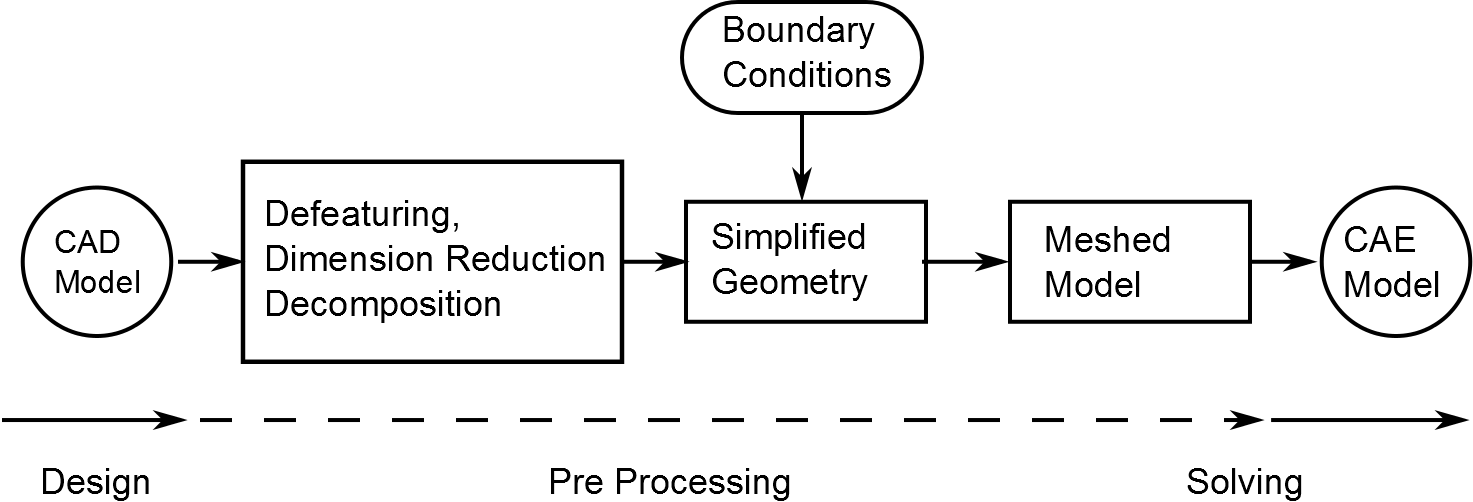
\includegraphics[width=0.9\linewidth]{..//Common/images/CADCAEGeneralProcess.png}
		\vspace{\abovecaptionskip}
		\caption{General Process (Source \cite{Tierney2013})}
		\label{CADCAEGeneralProcess}
	\end{figure}



\section{Model Simplification}

{\em Time-to-Market} being a crucial parameter for success of the product, development cycles have started reducing drastically. Simulations are now performed at the conceptual design stage itself. At this stage, expectation is of a quick assessment of the viability of the design and for this a detailed CAD model is not used but a more simplified, idealized one is analyzed. Unnecessary details add to complexities in mesh generation, and need more resources in terms of computational power-time for a relatively smaller gain in the accuracy of the results. So it is important to utilize simplified models that retain the important details and eliminate the irrelevant ones. The process of this conversion is known as Model Simplification (Figure \ref{ModelSimplification}). Even today it is a tedious and mostly a manual process taking significant amount of time \cite{Russ2012}. As elaborated by Thakur et. al.  in their survey paper \cite{Thakur2009} there have been many research efforts to automate the simplification process so far. However, at present, only limited automated capabilities exist requiring significant improvement \cite{Lee2009}.
	
%	\begin{wrapfigure}{l}{0.3\textwidth}
%	\centering
%	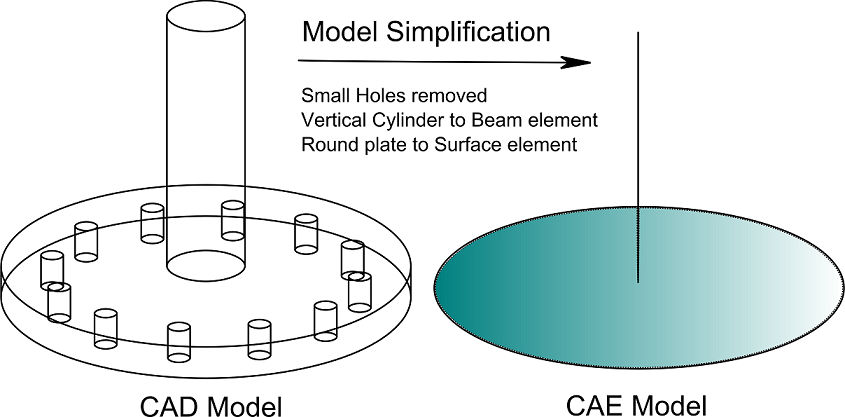
\includegraphics[scale=0.28]{..//Common/images/ModelSimplification.png}
%	\caption{Model Simplification}
%	\label{ModelSimplification}
%	\end{wrapfigure} 

	\begin{figure} [h]
		\centering
		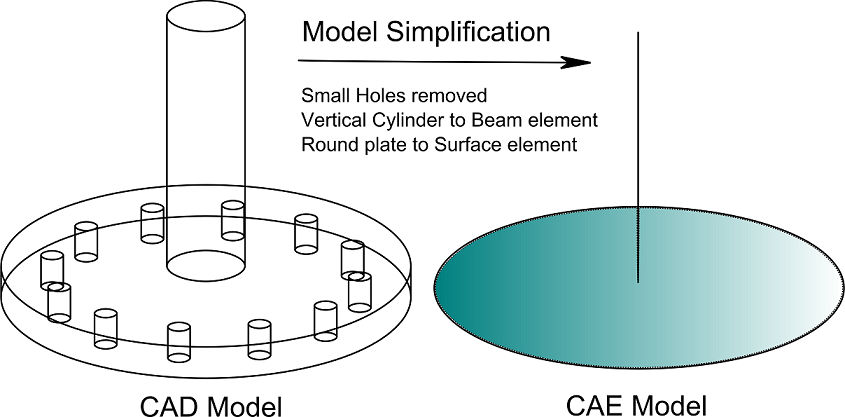
\includegraphics[width=0.9\linewidth]{..//Common/images/ModelSimplification.png}
		\vspace{\abovecaptionskip}
		\caption{Model Simplification consisting of both Global and Elemental idealization}
		\label{ModelSimplification}
	\end{figure}

	Model Simplification, according to Dabke \cite{Dabke1994}, can be classified into two parts, namely, Global and Element Idealization. Global Idealization deals with suppressing irrelevant features and takes advantage of the symmetry to analyze only a portion of the model. In Element Idealization, shapes like slender-bar, thin-wall are converted into lower dimension geometries. 

	Many Model Simplification  approaches do not utilize the feature information. They operate on the final CAD geometry as a whole and extract idealized shape. While doing so, connection of the analysis geometry with the features, corresponding semantics and the constraints that define the design model, are lost \cite{Smit2011}.
	
	
\section{Global Idealization using feature information}
	
	Global Idealization involves suppressing irrelevant features like small Holes, Fillets, Chamfers under certain parameters. Detection and suppression becomes far more straightforward with the features than doing similar process on just a Brep. One can leverage use of features such as Pattern, Mirror to detect symmetry and just keep master portion for the analysis. 

	 Lee \cite{Lee2005} proposed a method to reorder design features in the history tree and then re-execute the history of the reordered features up to the given level of simplification. Since re-evaluation of boundaries of a solid model is computationally heavy, he used cellular model for increasing the performance.

	To accomplish consistent simplification results independent of modeling history, it is necessary to recognize features to be removed directly from the final model.  As in design by features, the feature order governs the final result \cite{Russ2012}, Model Simplification done on such models may result in unacceptable results due to order dependencies between features. To avoid this, Woo \cite{Woo2009} proposed a new method which has subtractive features recognized directly from final solid. Thus during simplification process if these subtractive features are removed, result becomes far more acceptable.

\section{Element Idealization using feature information}

	\begin{figure}[h]
	\centering
	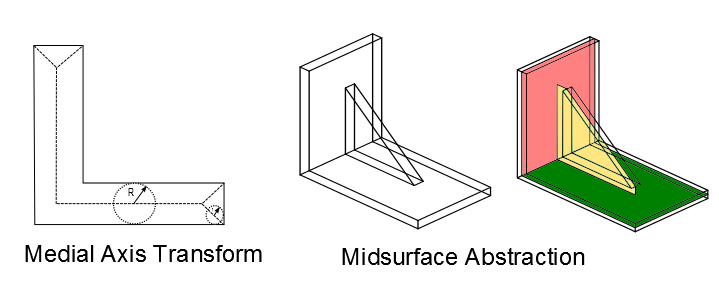
\includegraphics[width=0.9\linewidth]{..//Common/images//MAT_Midsurf.png}
	\caption{Midsurface Extraction Methods}
	\label{MATMidsurf}
	\end{figure}
	
	
%	\begin{wrapfigure}{l}{0.3\textwidth}
%	\centering
%	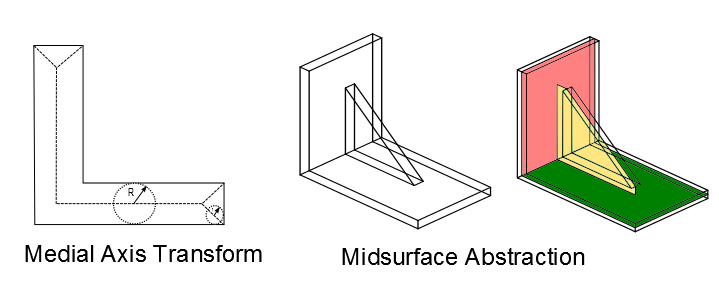
\includegraphics[scale=0.28]{..//Common/images//MAT_Midsurf.png}
%	\caption{Midsurface Extraction Methods}
%	\label{MATMidsurf}
%	\end{wrapfigure}

In Elemental Idealization, slender potions are abstracted to lines-curves where as for thin portions Midsurface is used as an idealized form. Such idealizations are expected to have proper connectivity  (no gaps) and they should follow shape of the base part. In Mid-surfacing techniques there are two broad categories namely, 'Medial Axis Transform (MAT)' and 'Midsurface Abstraction(MA)'.

MAT is a locus of the center of an inscribed disc of maximal diameter as it rolls around the object interior.  In 2D its called Medial Axis Curve (Figure \ref{MATMidsurf}) where as in 3D it is called Medial Surface. Major drawback of this method is that it creates unnecessary branches and its shape is smaller than the original corresponding faces. Plus there is major issue of perturbations, meaning slight change in the base geometry forces re-computation of MAT and the result could very well be different than the original.  Ramanathan \cite{Ramanathan2004} modified MAT method to remove erroneous branches. As most of the MAT algorithms are piecewise polygonal approximations, Fischer \cite{Elber1999} suggested method of parametric mid-curve which would have no branches and would represent shape of the parent curves.

MA (Figure \ref{MATMidsurf}) involves constructing 3D mid-surface for a part model by sewing the mid-surface patches obtained from each of the 'pairs of surfaces'. The surface-pairing approach has benefits over MAT techniques because the resultant geometry is cleaner and requires less reconstruction. However the surface pairing approach also has problems because it can be difficult to identify all of the surface pairs.

Hamdi et.al. \cite{Hamdi2005} used features for small details removal as well as talked about idealization in basic primitives liked Parallelepipeds, Cylinder and Wedge. 

Robinson et. al.  \cite{Robinson2006} utilize information contained in the CAD feature tree to locate sketches associated with suitable features in the model. Slender regions in the sketch are used to create sheet bodies representing thin regions of the component. 

Roland Stolt \cite{Stolt2005, Sunnersjo2005, Stolt2006} has developed idea of feature based Midsurface for a small set of features namely Pad and Pocket. He has elaborated how to treat negative volumes, fillets but did not elaborate much on how to create the mid-curves for complex 2D profiles. Also his work had restrictions like of using thin wall parts with preferably constant thickness and also did not provide thickness values on the Midsurface which is necessary for creating Shell elements.

	Smit \cite{Smit2011} linked CAD and CAE model on the basis of individual features. Method was developed to decide which feature gets abstracted to what level and which features can be ignored in the creation of analysis model. But even though individual features created their own abstraction, connecting them became a challenging task.
	
The above mentioned techniques do not elaborate much on how feature interactions are dealt with and also are based on extraction algorithm applied on the final shape. Many a times, due to complexity in recognizing forms, and due to complex interactions between them, Midsurface of the part does not follow its form and is not fully connected \cite{Sheen2008} . Solution could be, to create Midsurface while building the model itself.

In Features-based Solid Modeling, input feature-parameters are used to build tool-bodies and the whole part gets built using direct or indirect boolean of base and tool bodies. Creating Midsurface for individual tool bodies appears to be a more deterministic problem than recognizing the feature forms. With well-defined boolean operations, correct Midsurface connectivity can be ensured.  

\section{Literature Survey - Model Simplification}

tbd

%\section{Frequently Asked Questions}
%\subsection{What is Thin?}
%\subsection{Why not One Side?}
%\subsection{Why was it not done before?}
%\subsection{Whats so special about features?}
%
%\subsection{Autodesk Inventor Sheet Metal has following features}
%
%\begin{table}[!h]
%\begin{tabular}[h]{@{}l l l l @{}}
%
%\textcolor{yellow}{AliasFreeForm}	&
%\textcolor{green}{Bend} &
%\textcolor{green}{BendPart} &
%\textcolor{blue}{Boss} \\
%
%\textcolor{yellow}{BoundaryPatch} &
%\textcolor{blue}{Chamfer} &
%\textcolor{cyan}{CircularPattern} &
%\textcolor{cyan}{Client} \\
%
%\textcolor{blue}{Coil} &
%\textcolor{blue}{Combine} &
%\textcolor{green}{ContourFlange} &
%\textcolor{green}{ContourRoll} \\
%
%\textcolor{green}{CoreCavity} &
%\textcolor{green}{CornerChamfer} &
%\textcolor{green}{Corner} &
%\textcolor{green}{CornerRound} \\
%
%\textcolor{blue}{Cut} &
%\textcolor{cyan}{Decal} &
%\textcolor{blue}{Deleteface} &
%\textcolor{blue}{Emboss} \\
%
%\textcolor{yellow}{Extend} &
%\textcolor{blue}{Extrude} &
%\textcolor{blue}{FaceDraft} &
%\textcolor{green}{Face} \\
%
%\textcolor{blue}{FaceOffset} &
%\textcolor{blue}{Fillet} &
%\textcolor{green}{Flange} &
%\textcolor{green}{Fold} \\
%
%\textcolor{green}{Grill} &
%\textcolor{green}{Hem} &
%\textcolor{blue}{Hole} &
%\textcolor{green}{Knit} \\
%
%\textcolor{green}{Lip} &
%\textcolor{green}{LoftedFlage} &
%\textcolor{blue}{Loft} &
%\textcolor{yellow}{Midsurface} \\
%
%\textcolor{cyan}{Mirror} &
%\textcolor{blue}{MoveFace} &
%\textcolor{cyan}{Move} &
%\textcolor{cyan}{NonParametricBase} \\
%
%\textcolor{green}{PunchTool} &
%\textcolor{cyan}{RectangularPattern} &
%\textcolor{green}{Refold} &
%\textcolor{blue}{ReplaceFace} \\
%
%\textcolor{green}{Rest} &
%\textcolor{blue}{Revolve} &
%\textcolor{green}{Rib} &
%\textcolor{green}{Rip} \\
%
%\textcolor{blue}{RuleFillet} &
%\textcolor{blue}{Sculpt} &
%\textcolor{blue}{Shell} &
%\textcolor{green}{SnapFit} \\
%
%\textcolor{cyan}{Split} &
%\textcolor{blue}{Sweep} &
%\textcolor{yellow}{Thicken} &
%\textcolor{blue}{Thread} \\
%
%&\textcolor{cyan}{Trim} &
%\textcolor{green}{Unfold} &\\
%\\
%\textcolor{yellow}{Surface} &
%\textcolor{blue}{Solid} &
%\textcolor{green}{SheetMetal} &
%\textcolor{cyan}{Others}\\
%
%\end{tabular}
%\end{table}

\section{Conclusions of Literature Survey}
tbd

